\chapter{Results}
\label{cha:results}

Present your results in an objective way. Use tables and charts, but do not
forget to also include a summary in text form. Do not interpret your results.

This chapter presents the results. Note that the results are presented
factually, striving for objectivity as far as possible.  The results
shall not be analyzed, discussed or evaluated.  This is left for the
discussion chapter.

In case the method chapter has been divided into subheadings such as
pre-study, implementation and evaluation, the result chapter should
have the same sub-headings. This gives a clear structure and makes the
chapter easier to write.

In case results are presented from a process (e.g. an implementation
process), the main decisions made during the process must be clearly
presented and justified. Normally, alternative attempts, etc, have
already been described in the theory chapter, making it possible to
refer to it as part of the justification.


\begin{table}[]
    \centering
    \caption{Model result on train data.}
    \label{tab:train-table}
    \begin{tabular}{@{}llllll@{}}
    \toprule
    Model                         & TP             & FP            & FN            & TN             & Accuracy      \\ \midrule
    Dummy Classifier (stratified) & 24015          & 24172         & 24179         & 24221          & 0.50          \\
    Multinomial Naive Bayes       & 41980          & 6207          & 5356          & 43044          & 0.88          \\
    Linear SVM (SGD)              & 40443          & 7744          & 3350          & 45050          & 0.89          \\
    Logistic Regression           & \textbf{42155} & \textbf{6032} & 3049          & 45351          & \textbf{0.91} \\
    KNN                           & 34689          & 13498         & \textbf{2900} & \textbf{45500} & 0.83          \\
    Random Subspaces (SVM)        & 38322          & 9865          & 6028          & 42372          & 0.84          \\ \midrule
    \textbf{True Classification}  & \textbf{48187} & \textbf{0}    & \textbf{0}    & \textbf{48400} & \textbf{}    
    \end{tabular}
\end{table}


\begin{table}[]
    \centering
    \caption{Model result on test data.}
    \label{tab:test-table}
    \begin{tabular}{@{}llllll@{}}
    \toprule
    Model                         & TP             & FP            & FN            & TN             & Accuracy      \\ \midrule
    Dummy Classifier (stratified) & 10480          & 10324         & 10276         & 10315          & 0.50          \\
    Multinomial Naive Bayes       & \textbf{18042} & \textbf{2762} & 2841          & 17750          & \textbf{0.86} \\
    Linear SVM (SGD)              & 16851          & 3953          & 1794          & 18797          & \textbf{0.86} \\
    Logistic Regression           & 17084          & 3720          & 2015          & 18576          & \textbf{0.86} \\
    KNN                           & 13461          & 7343          & \textbf{1709} & \textbf{18882} & 0.78          \\
    Random Subspaces (SVM)        & 16446          & 4358          & 3005          & 17586          & 0.82          \\ \midrule
    \textbf{True Classification}  & \textbf{20804} & \textbf{0}    & \textbf{0}    & \textbf{20591} & \textbf{}    
    \end{tabular}
\end{table}



\begin{table}[]
    \centering
    \caption{Majority Voting on test data.}
    \label{tab:voting-table}
    \begin{tabular}{@{}llllll@{}}
    \toprule
    Model                  & TP    & FP   & FN   & TN    & Accuracy \\ \midrule
    Majority Voting     & 17210 & 3594 & 1891 & 18700 & 0.87     \\ \bottomrule
    \end{tabular}
\end{table}



\begin{table}[]
    \centering
    \caption{Model result on validation data.}
    \label{tab:validation-table}
    \begin{tabular}{@{}llllll@{}}
    \toprule
    Model                        & TP             & FP            & FN            & TN             & Accuracy      \\ \midrule
    Multinomial Naive Bayes      & \textbf{8839}  & \textbf{1828} & 2945          & 10721          & 0.80          \\
    Linear SVM (SGD)             & 8137           & 2530          & \textbf{1746} & \textbf{11920} & 0.82          \\
    Logistic Regression          & 8342           & 2325          & 2092          & 11574          & 0.82          \\
    Majority Voting              & 8420           & 2247          & 1914          & 11752          & \textbf{0.83} \\ \midrule
    \textbf{True Classification} & \textbf{10667} & \textbf{0}    & \textbf{0}    & \textbf{13666} &              
    \end{tabular}
\end{table}



\begin{figure}[h]
    \caption{Demo plot}
    \centering
    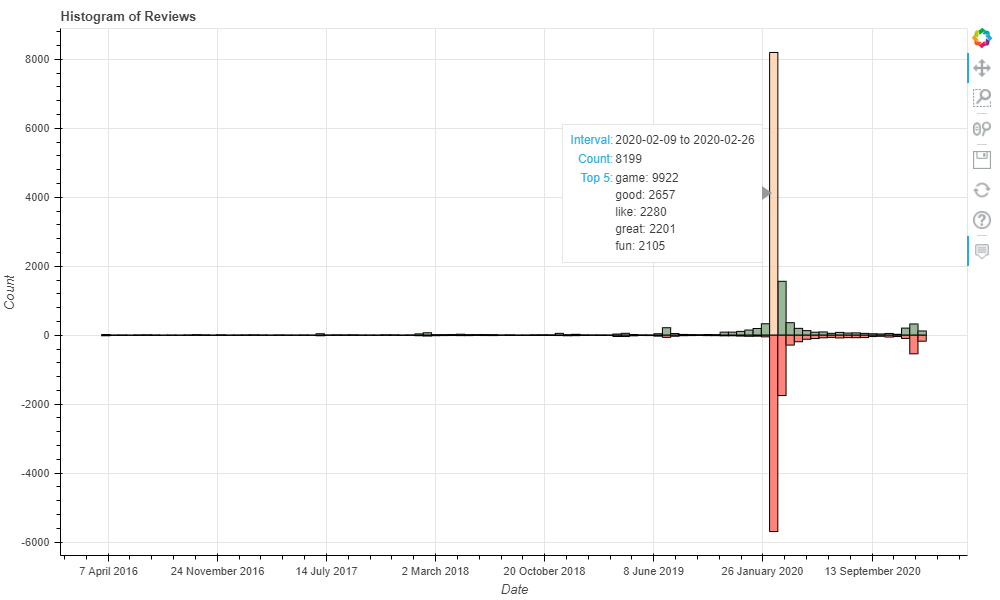
\includegraphics[width=1\textwidth]{../plots/demo.png}
\end{figure}